% SPDX-License-Identifier: Apache-2.0
% SPDX-FileCopyrightText: Copyright contributors to the vLLM project
\documentclass[11pt,a4paper]{article}
\usepackage[margin=24mm,headheight=15pt]{geometry}
\usepackage[T1]{fontenc}
\usepackage{lmodern}
\usepackage{microtype}
\usepackage{amsmath}
\usepackage{booktabs,longtable,tabularx,array}
\usepackage{xcolor}
\usepackage{enumitem}
\usepackage{fancyhdr}
\usepackage{fancyvrb}
\usepackage{tikz}
\usetikzlibrary{arrows.meta,positioning}
\usepackage{xurl}
\usepackage{hyperref}
\definecolor{accent}{HTML}{174A6B}
\definecolor{muted}{HTML}{53616B}
\definecolor{pale}{HTML}{EDF4F8}
\hypersetup{colorlinks=true,linkcolor=accent,urlcolor=accent,citecolor=accent,
  pdftitle={AMD vLLM CI and deployment: a shared runtime and commit wheel},
  pdfauthor={Local engineering proposal},bookmarksnumbered=true}
\urlstyle{tt}
\newcommand{\file}[1]{\nolinkurl{#1}}
\newcommand{\term}[1]{\texttt{\detokenize{#1}}}
\newcolumntype{L}[1]{>{\raggedright\arraybackslash}p{#1}}
\DefineVerbatimEnvironment{Code}{Verbatim}{fontsize=\footnotesize,
  frame=single,rulecolor=\color{muted},framesep=3mm}
\setlength{\parindent}{0pt}
\setlength{\parskip}{6pt plus 1pt}
\setlength{\emergencystretch}{3em}
\setlist{nosep,leftmargin=*,topsep=5pt}
\renewcommand{\arraystretch}{1.18}
\pagestyle{fancy}
\fancyhf{}
\fancyhead[L]{\small AMD vLLM runtime and CI}
\fancyhead[R]{\small Local migration proposal}
\fancyfoot[C]{\thepage}
\fancypagestyle{plain}{\fancyhf{}\fancyfoot[C]{\thepage}}
\begin{document}

\hypersetup{pageanchor=false}
\begin{titlepage}
\raggedright
\vspace*{17mm}
{\color{accent}\Large Engineering design and implementation report\par}
\vspace{10mm}
{\Huge\bfseries AMD vLLM CI\par and deployment\par}
\vspace{8mm}
{\LARGE A shared dependency runtime\par and one wheel per commit\par}
\vspace{12mm}
{\large Design baseline: TheRock / ROCm 10 PR \#58761\par}
\vspace{3mm}
\file{92e64dd45470e12fadaa56081facc370f552da88}\par
\vspace{8mm}
10 October 2026\par
\vfill
\colorbox{pale}{\parbox{0.94\textwidth}{\raggedright\vspace{3mm}
\textbf{Review status.} This report describes the local implementation in
\file{/app/vllm}, its measured experiments, and the work required for rollout.
The assumed prerequisite PR lands first. The candidate has not replaced the
production pipeline, and a complete ROCm 10 image has not been built or validated
on GPUs in this environment.\vspace{3mm}}}\par
\vspace{7mm}
{\small This report records local development and experiments. Source and report
publication is a separate review step; no container images or pipelines were
published during evaluation.\par}
\end{titlepage}

\pagenumbering{roman}
\hypersetup{pageanchor=true}
\tableofcontents
\clearpage
\pagenumbering{arabic}

\section{Decision, scope and current status}

The proposed deployment contract has two independently reusable inputs:
\textbf{one immutable dependency runtime image} and \textbf{one exact vLLM wheel
for each commit}. The OpenAI serving image combines those inputs. CI starts
from that runtime digest and installs that same wheel with the same offline
installer. Frozen test tools and a thin workspace remain separate bundles.

The architectural change is to stop treating \term{base}, \term{ci_base}, a
per-commit CI image, and an independently resolved serving image as separate
consumer environments. Dependency compilation is a refresh activity. Native
and Rust compilation for vLLM is a builder activity. Neither requires another
image contract that every GPU worker must pull.

The local implementation uses the two existing primary ROCm 10 recipes:
\file{docker/Dockerfile.rocm_base} and \file{docker/Dockerfile.rocm}.
The requested underscore in \term{rocm_base} is retained. The four additional
runtime-build, runtime, commit and deployment Dockerfiles introduced during
earlier exploration were removed. Existing ROCm 7.2 and other compatibility
recipes remain inherited from the baseline.

This is a \emph{migration candidate}, with explicit boundaries between working
local mechanisms and proposed fleet integration:

\begin{tabularx}{\textwidth}{L{30mm}X}
\toprule
Status & What it means in this checkout \\
\midrule
Implemented locally & Artifact locks, dependency-producer plans, offline build
targets, shared installer, worker handoff, pipeline renderer, cache-safe payload
groups, local secret audit, and compatible legacy-path fixes. \\
Exercised locally & Focused tests, small real Python-wheel fixtures, OCI
reachability and secret fixtures, codec measurements, static Bake/recipe checks,
and host ROCm file-access tracing. \\
Not executed & A complete ROCm 10 dependency build, complete offline vLLM
native/Rust build, actual serving-image canary, GPU model tests, and independent
cold image reproducibility checks. \\
Not integrated & Production artifact transport, digest catalog, retention
leases, delayed worker upload, all NIC/test profiles, and retirement of legacy
consumer routes. \\
\bottomrule
\end{tabularx}

The default legacy HCL, Buildkite build scripts and independent
\term{final_common} serving resolver still run their inherited paths.
Adding the candidate targets does not establish a production cutover.
The report describes both the intended end state and the concrete local changes
needed to evaluate it without publishing anything.

\section{Starting point and problems to solve}

\subsection{TheRock is the prerequisite}

The review baseline is the exact PR \#58761 head stated on the cover, rather
than the old source-oriented ROCm stack. The PR makes ROCm 10 SDK and PyTorch
wheels the default and retains a ROCm 7.2 compatibility path~\cite{therock}.
It does not make every framework an upstream wheel: MoRI, FlashAttention,
AITER, custom Triton and patched ROCr/CLR still have source-built components.
The second recipe also contains NIXL/UCX, DeepEP, LMCache, rdma-core, TorchCodec
and a ROCm fastsafetensors extension.

These source exceptions become dependency artifact producers. Their validated
wheels and required system libraries join the locked runtime closure. An
upstream wheel can replace a producer only after the same ABI, architecture and
GPU checks pass. Assuming that all exceptions disappear with TheRock would
leave a deployment that differs from the baseline's patched image.

The inherited test path also overlays checkout code, including
\file{vllm/v1}, onto an installed wheel. Meanwhile serving resolves dependencies
separately. A test passing against that environment does not prove that the
serving artifact contains the tested code or dependency versions.

\subsection{Issue coverage}

The cited reports identify related but distinct bottlenecks. The following
table separates a proposed remedy from proof that it has fixed the fleet.

\begin{longtable}{L{31mm}L{57mm}L{60mm}}
\toprule
Concern & Proposed change & Evidence and remaining work \\
\midrule
\endhead
ROCm gzip omission, issue \#28656 comment~\cite{compressionissue} & Use zstd
on the compatible old path; select canonical encoding for the new runtime. &
Local decode probes support the choice. Actual daemon pull/unpack A/B testing
is still required. \\
Volatile ROCm 10 layer, issue \#60258~\cite{karl} & Select a runtime by content
key; lock exact wheel bytes; remove commit/build identifiers from dependency
identity; make installation deterministic. & File metadata, bytecode and uv
ctime churn were demonstrated. They are candidate mechanisms, not a proven
root cause of the reported entire layer. \\
Old infra proposal \#447~\cite{infra} & Preserve conditions/concurrency and
select the same image in native and DinD paths before scheduling workers. &
Local vLLM renderer implements its side. Infra changes were prototyped in a
removed clone and require a separate follow-up. \\
Too many deployment recipes and wrappers & Add targets to two existing
Dockerfiles; use one worker entrypoint and one installer. & Additional
Dockerfiles and two added shell wrappers were removed. Legacy scripts remain
until validated cutover. \\
Disk growth and image contents & Separate builder GC, worker snapshot GC and
artifact retention; evaluate slimming from workload traces. & GC policy file
was supplied; isolated OCI pruning was exercised. No live daemon pruning or trace-based
runtime deletion is active. \\
Tokens and secrets & Audit every exported OCI layer plus config/history and
embedded wheels before local assembly is accepted. & Mandatory gate on the new
local assembly path; successful planted-secret fixtures. Legacy publishing paths
are not yet gated. \\
\bottomrule
\end{longtable}

Karl's report describes a roughly 9.5--10.6 GiB changing ROCm 10 top layer, with
0.2\% pairwise sharing compared with 86.5\% in the ROCm 7.2 lineage, and a
12.8-fold median pull-duration difference~\cite{karl}. Those are reported fleet
observations, not measurements produced by this local implementation.
Reusing an already validated runtime digest avoids both retransferring and
reapplying its unchanged filesystem; compression alone addresses only part of
the cost.

\clearpage
\section{The simplified deployment graph}

\begin{center}
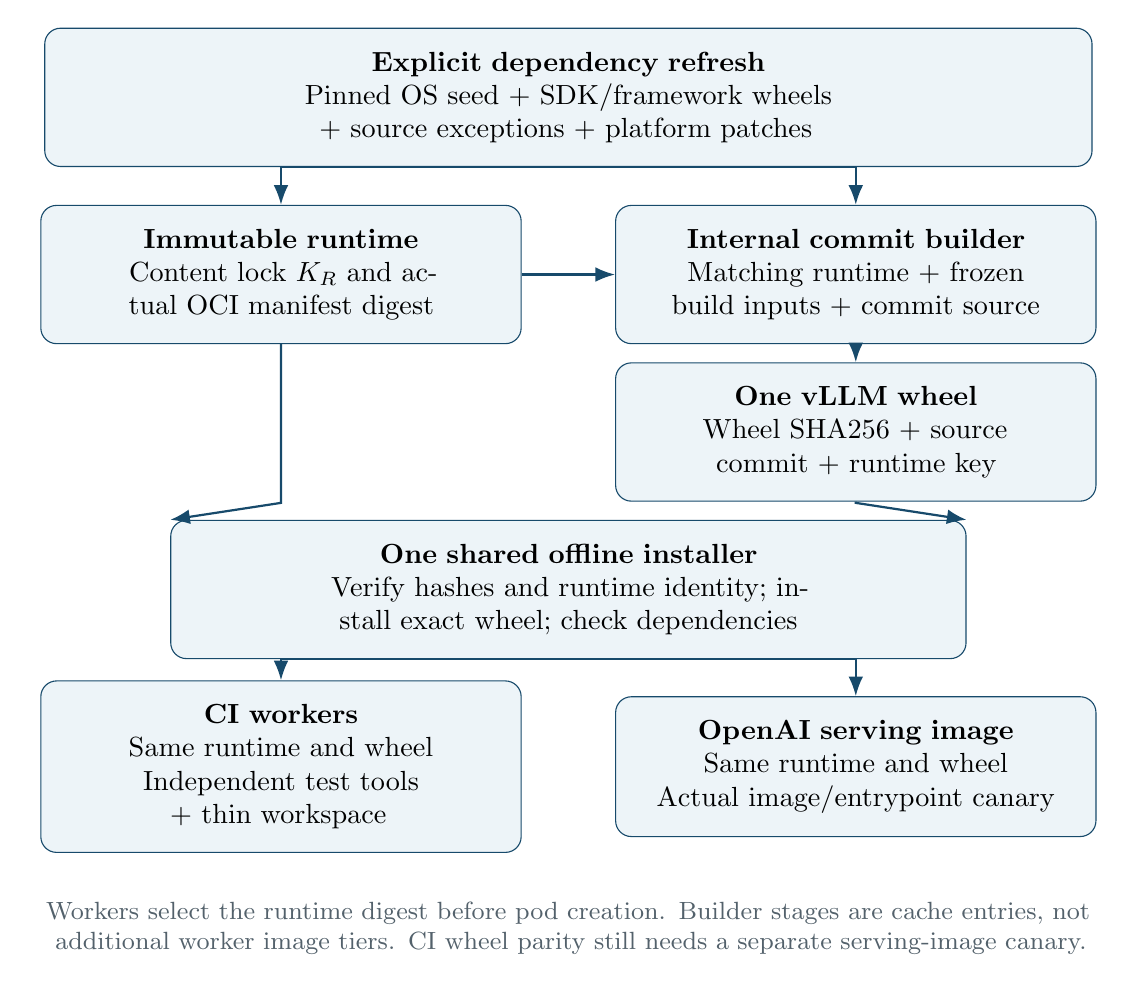
\begin{tikzpicture}[
  box/.style={draw=accent,rounded corners=2mm,fill=pale,align=center,
    text width=55mm,minimum height=16mm,inner sep=3mm},
  wide/.style={box,text width=127mm},
  arrow/.style={-{Latex[length=2.5mm]},thick,draw=accent},
  note/.style={font=\small\color{muted},align=center}]
\node[wide] (refresh) at (0,0) {\textbf{Explicit dependency refresh}\\
Pinned OS seed + SDK/framework wheels + source exceptions + platform patches};
\node[box] (runtime) at (-3.65,-2.25) {\textbf{Immutable runtime}\\
Content lock $K_R$ and actual OCI manifest digest};
\node[box] (build) at (3.65,-2.25) {\textbf{Internal commit builder}\\
Matching runtime + frozen build inputs + commit source};
\node[box] (wheel) at (3.65,-4.25) {\textbf{One vLLM wheel}\\
Wheel SHA256 + source commit + runtime key};
\node[wide,text width=95mm] (install) at (0,-6.25)
{\textbf{One shared offline installer}\\
Verify hashes and runtime identity; install exact wheel; check dependencies};
\node[box] (ci) at (-3.65,-8.5) {\textbf{CI workers}\\
Same runtime and wheel\\Independent test tools + thin workspace};
\node[box] (serve) at (3.65,-8.5) {\textbf{OpenAI serving image}\\
Same runtime and wheel\\Actual image/entrypoint canary};
\draw[arrow] (refresh.south) -| (runtime.north);
\draw[arrow] (refresh.south) -| (build.north);
\draw[arrow] (runtime.east) -- (build.west);
\draw[arrow] (build) -- (wheel);
\draw[arrow] (runtime.south) -- (-3.65,-5.15) -- (install.north west);
\draw[arrow] (wheel.south) -- (3.65,-5.15) -- (install.north east);
\draw[arrow] (install.south) -| (ci.north);
\draw[arrow] (install.south) -| (serve.north);
\node[note,text width=135mm] at (0,-10.55) {Workers select the runtime digest
before pod creation. Builder stages are cache entries, not additional worker
image tiers. CI wheel parity still needs a separate serving-image canary.};
\end{tikzpicture}
\end{center}

\subsection{Consumers, stages and layers are different things}

\begin{tabularx}{\textwidth}{L{38mm}X}
\toprule
Boundary & Contract \\
\midrule
Worker image & A single immutable runtime selected by its actual digest. \\
Commit artifact & Exactly one vLLM wheel bound to that runtime and source SHA. \\
Serving image & Runtime plus the same wheel; its image configuration is tested
separately. \\
Internal build stages & Source producers, OS seed, native compiler, Rust builder
and packaging stages stay on dedicated builders. \\
OCI layers & Separate stable payload groups retain compressed-blob reuse. They
do not create additional worker environments. \\
\bottomrule
\end{tabularx}

Squashing all payloads into a single layer would make small changes invalidate a
large transfer. The candidate keeps SDK, PyTorch core, Triton and remaining Python
files in separate groups, then applies the small platform sidecar afterward.
PyTorch core here means \term{torch}, \term{torchgen} and their metadata;
Torchvision and torchaudio remain in the general Python group.

The splitter preserves paths, bytes, modes, symlinks and hardlinks by moving
payloads before final copies. Changes in general Python dependencies should
leave the SDK/core framework groups reusable. This behavior was checked with
filesystem fixtures; the actual compressed layer boundary still needs two
independent full runtime builds.

The serving target is a derived deployment product, not another independently
resolved dependency tier. Similarly, \term{deployment-test} is a local evaluation
view rather than a mandatory image that every CI worker pulls.

\subsection{Target organization in two recipes}

\begin{tabularx}{\textwidth}{L{54mm}X}
\toprule
Recipe & Candidate target families \\
\midrule
\file{docker/Dockerfile.rocm_base} &
\term{seed-os}, \term{rdma-build}, \term{runtime-seed}, \term{resolve},
\term{validate}, \term{export-artifacts}; then \term{runtime-install} and
\term{runtime}. \\
\file{docker/Dockerfile.rocm} &
\term{wheel-build-tools}, Rust cache/build, native build, package and
\term{wheel-export}; then \term{deployment} and \term{deployment-test}. \\
\bottomrule
\end{tabularx}

The candidate groups are fenced in the recipes so their hashes can be scoped.
The inherited stages and default target selection remain unchanged during
migration. This consolidation makes the candidate easier to review; deleting
the old targets before canaries pass would prematurely remove the rollback path.

\section{Content identity and caching}

\subsection{Runtime lock}

The lock is a canonical JSON record with a SHA256 key. Conceptually,
\begin{align*}
K_R &= \operatorname{SHA256}(\operatorname{canonicalJSON}(R)),\\
R &= \{\text{schema, OS digest, cp312 ABI, GPU arches, epoch, wheel records,}\\
  &\hspace{10mm}\text{platform records, scoped recipe, installer/splitter hashes,
  encoding}\}.
\end{align*}
Each wheel record contains its exact filename, normalized distribution name,
version, byte size, SHA256, import roots and console scripts. The filename's
identity must agree with the wheel's METADATA. Platform records include file
contents, paths, modes and symlink targets. The sidecar permits only the declared
\file{/opt/venv} and \file{/etc} structure and rejects escaping links or special
files.

The runtime lock excludes a vLLM commit wheel, build UUID and current application
commit. Source commits, patches, toolchain inventories and validation logs are
recorded separately as provenance. A provenance-only change must not generate a
new runtime content key when the actual deployment inputs are identical.

Runtime identity hashes the fenced runtime group, the digest-pinned Dockerfile
frontend and its global \term{OS_IMAGE} argument. The commit-build prerequisite
lock separately hashes its fenced group, frontend and \term{RUNTIME_IMAGE}
argument. Editing an unrelated deployment or producer target therefore does not
invalidate the runtime lock. Relevant assembly changes still invalidate it.

Encoding is explicit: OCI media types, zstd and the selected level. Different
compressed bytes have different registry/content-store digests even when their
uncompressed diffID is equal. A codec change is a deliberate runtime refresh.
It must not happen implicitly at each commit export.

\subsection{Application and test locks}

A commit lock accepts exactly one wheel named vLLM. It binds that wheel to the
runtime key and a complete 40-hex source commit. Handoff checks reject a mismatch
between wheel provenance and the thin test checkout.

Test tools have a separate lock bound to the runtime. They may not overlap a
deployed distribution, import root or console script, including vLLM itself.
Keeping their install target outside \file{/opt/venv} avoids turning a test
dependency upgrade into a large runtime refresh.

Named hashed requirements use the form
\term{package==version --hash=sha256:...}. They are resolved only against the
local flat wheelhouse. Direct wheel paths are avoided because their locations
can become \file{direct_url.json} metadata and introduce path-dependent bytes.

\subsection{Expected cache behavior}

\begin{tabularx}{\textwidth}{L{48mm}X}
\toprule
Change & Expected result \\
\midrule
Only vLLM code changes & Same runtime digest; new commit wheel and small
application-derived serving layers. \\
Only tests/tools change & Same runtime; new test tools or source bundle as
needed. Relevant commit artifact may remain reusable. \\
Only build UUID changes & Same runtime content identity. \\
Only provenance text changes & Same runtime identity when artifact bytes and
assembly inputs remain identical. \\
One Python dependency changes & New runtime key; large SDK/PyTorch-core/Triton
groups can remain reusable if their bytes and metadata remain identical. \\
SDK, OS seed, platform patch or ABI changes & New runtime lock; rebuild and
validate the affected groups and deployment closure. \\
Compression level changes & New encoded blob identity and runtime lock. \\
\bottomrule
\end{tabularx}

On a lock hit, the future catalog selects the previously validated runtime
digest directly. It should not reinstall identical dependencies to discover the
same content again. That catalog and its validation state are integration work.

For a node that already holds the runtime and test tools, the intended per-commit
transfer is the wheel plus changed workspace/test artifacts. A cold node also
needs the runtime. Approximate network demand over $N$ nodes is
\[
 B \simeq N_{\mathrm{cold}} B_R
       + N B_W + B_{\mathrm{changed\ tools/workspaces}},
\]
with further savings when the artifact transport shares downloads between jobs.
The equation states the cache objective, not a measured fleet result. Real
vLLM wheel sizes must be measured before promising a particular megabyte-sized
delta. Model weights and test datasets are outside this artifact pipeline and
may still require network access.

\section{Dependency refresh and runtime assembly}

\subsection{Refresh is the network boundary}

\file{tools/vllm-rocm/produce_runtime.py} constructs a local Bake graph from the
assumed PR's source producers. It exports an OS seed, a complete wheelhouse,
platform patches and provenance. It does not need the old \term{ci_base} or
test image as a distributed input.

Stable/nightly indexes are consulted only during explicit refresh. The producer
collects source-built framework/native wheels and downloads the remaining binary
closure. A URL or version string is insufficient: nightly bytes can change under
the same version. The frozen closure hashes the actual bytes and includes
otherwise indirect dependencies, such as the MoRI web/runtime dependencies.

The first implemented provider is CX7, with a shared server GPU profile
\term{gfx90a;gfx942;gfx950}. AITER and DeepEP retain their declared narrower
\term{gfx942;gfx950} support. AINIC, Broadcom, Mamba/causal-conv and dependency
compatibility variants need separate validated provider/profile inputs. They
cannot be silently omitted from a fleet migration.

\subsection{OS and platform closure}

The initial seed is Ubuntu 22.04 with Python 3.12, venv support, loader utilities,
FFmpeg/media dependencies and required system/RDMA libraries. rdma-core is pinned
to commit \file{31af04ec84378724cb6256814d4ffde359a7123b}; its exported runtime
removes man pages, static libraries and CMake package files. The seed retains
compiler/Python development packages needed by JIT assumptions. The SDK retains
development files until GPU validation supports further removal.

APT refresh records an inventory, but it is not yet backed by a frozen package
snapshot. Pinning the resulting seed manifest digest stabilizes downstream
assembly; rebuilding that seed independently from live APT inputs is a different
reproducibility requirement. Ubuntu 24.04 would be a separate compatibility
experiment.

The platform sidecar preserves the baseline's patched ROCr/CLR files, SDK links,
loader initialization, Kineto/profiler workaround and amdsmi behavior. It is
applied after SDK wheel installation and initialization. Known gfx90a xnack
kpack payloads are removed in their owning wheels with corresponding RECORD
updates. This targeted producer trim is distinct from unvalidated trace-based
slimming.

The proposed fresh-seed validator imports Torch/Triton, checks SDK clang and
runs host x86 ELF dependency checks after patches. It avoids validating only in
the larger producer filesystem, where missing runtime dependencies can be hidden.
These full-stack validation steps are implemented in recipes but have not run
on a complete ROCm 10 candidate here.

\subsection{Offline assembly}

The assembler consumes already frozen wheelhouses and a digest-selected OS seed.
Its install uses pip with no index, no dependency resolution, no compilation,
required hashes and a local wheelhouse. Missing wheels fail instead of reaching
the network. The final runtime records \file{/opt/venv/.vllm-runtime-key},
runs loader/dependency checks and copies the shared installer under
\file{/opt/vllm-rocm}.

The splitter prepares the four payload groups before their final COPY layers.
The small platform patch is copied afterward, preventing a small patch change
from replacing a large SDK layer. BuildKit timestamp rewriting and a fixed
artifact epoch constrain filesystem metadata churn~\cite{exporters}.

Candidate runtime, commit and deployment \term{RUN} steps disable networking.
Dependency refresh remains networked. Resolving the pinned frontend or a base
image can still need an initial read unless it is preseeded or supplied through
verified local OCI contexts~\cite{contexts}. ``Offline installation'' is therefore
a precise build-step property, not a claim that the whole refresh lifecycle is
network-free.

\section{One commit build and one shared installation path}

\subsection{Builder-only prerequisites}

\file{tools/vllm-rocm/build_commit.py} freezes a separate input bundle:
\begin{itemize}
\item Python build wheels, without replacing the runtime GPU frameworks;
\item the complete native development \file{.deb} closure;
\item an installed Rust toolchain, Cargo vendor configuration/crates;
\item pinned Triton-kernels source and input provenance.
\end{itemize}
It checks tree contents/modes, architectures, required pins and runtime identity,
then creates separate native, Rust, packaging and tiny version contexts. The
native and Rust outputs join only at wheel packaging. The export contains the
vLLM wheel, not a new worker compiler image.

The Rust cache stage uses a constant build version, followed by a small exact
version stamp derived from host Git/SCM identity. Reuse is scoped to source-
consistent target trees; a persistent target cache is not blindly carried across
unrelated source revisions. The packaging stage keeps the baseline's
\term{PYTORCH_ROCM_ARCH} selection so per-device TheRock extras are preserved.

All candidate compile/install steps are offline. Preparing the real prerequisite
closure remains unfinished. A host \term{cargo metadata --frozen} probe failed
because the pinned zeromq Git revision was not available offline. This is evidence
that Cargo vendoring is a required missing input, not evidence that the complete
offline wheel build succeeded.

\subsection{The installer is the deployment contract}

\file{tools/vllm-rocm/install_artifacts.py} is used by both deployment assembly
and CI workers. Before pip runs, it checks:
\begin{enumerate}
\item the runtime marker and artifact lock identity;
\item every wheel's hash/size and the exact wheelhouse membership;
\item the named hashed requirements against that lock;
\item for a commit, the selected vLLM wheel SHA; for tools, its separate key
and an absolute, new target directory.
\end{enumerate}

It clears inherited pip configuration and Python path/home overrides, forces a
local no-index install with no dependencies or bytecode compilation, then runs
\term{pip check}. The commit installation uses \term{--force-reinstall} so a
different wheel with the same version replaces the old code. The old wheel marker
is removed after validation and before installation; the new marker is written
only after checks pass. A failed replacement must not retain a misleading success
marker.

Test tools install into an independent target. The worker owns lock-protected
temporary directories and atomic promotion of a verified tools cache. Candidate
fixtures confirmed isolated tools, rejection before installation and matching
normalized installed bytes across differing source wheelhouse paths.

\subsection{What deployment parity proves}

The runtime digest, installed vLLM wheel bytes and installer behavior match across
the two consumers. Workers prevent checkout \term{vllm} modules from shadowing
the installed wheel, and preflight checks confirm import location and markers.

This is installed-artifact parity. It does not test image ENTRYPOINT, CMD,
environment or serving-image startup automatically. The \term{deployment} target
sets \term{vllm serve}; a canary must run the actual exported image and exercise
the OpenAI API. Compatibility tests that intentionally replace Transformers or
another deployment dependency need declared profiles and cannot count as parity
tests for the original lock.

\section{CI handoff, worker launch and remaining infra work}

\subsection{Select the image before scheduling}

Kubernetes chooses a pod image before job commands run. The actual runtime digest
must therefore be known before worker steps are rendered. A shell command inside
an already scheduled pod cannot correct an earlier floating-image selection.

\term{local_runtime.py pack} writes a schema-1 handoff binding build ID, source
commit, producer step, runtime image/key, exact wheel hash, and the paths/hashes of
wheel, test-tools and source archives. Wheel bundles use uncompressed tar because
the wheels are already ZIP-compressed. Source/tests use deterministic gzip tar
with fixed metadata. The thin workspace includes selected tests, tools,
benchmarks, examples and configuration; it excludes the root vLLM package.

\file{.buildkite/scripts/rocm/runtime-pipeline.py} consumes an already selected
pipeline and the handoff. It emits worker/manual steps, maps legacy builder
dependencies to the single producer, pins the same digest in native and DinD
launch paths, and preserves conditions, concurrency, parallelism, plugins and
manual dependencies. It rejects selected job-time dependency/source mutations
with a migration report instead of silently running a different environment.

Rendering the real declarations from the assumed baseline identified 225 AMD
workers: 192 passed this declaration mutation screen and 33 required migration.
This count is a configuration audit, not a count of successful executed tests.
Completion/chat serving and LoRA canary YAML were emitted locally only.

\subsection{One worker entrypoint}

\file{.buildkite/scripts/rocm/runtime_worker.py --launch} handles native/DinD
dispatch, verified artifact extraction, temporary workspace preparation, offline
installation, preflight and test execution. Its launcher uses only the Python
standard library. Native jobs use the runtime's Python; DinD launches the exact
digest with the required devices/mounts and a controlled environment-name list.
Exit status and cleanup are preserved.

The two newly introduced worker/deployment-test shell wrappers were removed.
This reduces duplicated launch/install logic, but the legacy shell surface is
not yet retired. The utility modules remain distinct because dependency refresh,
commit compilation, artifact inspection and worker execution have different
inputs and trust boundaries.

\subsection{What is still outside the local renderer}

The artifact root must already be available to workers. A production shared or
prefetched store, its cache protocol, delayed bootstrap upload and runtime
lock-to-digest catalog are not implemented. Retention also needs active-job leases
so a running job cannot lose referenced bundles.

The separate ci-infra follow-up must preserve Buildkite \term{if}, concurrency
and concurrency groups throughout its renderers; use the same build-scoped image
in native/DinD paths during transition; support a validated digest override; and
serialize main-only promotion. The 540-minute rebuild timeout already exists in
the examined main baseline; it should not be advertised as a new fix copied from
the old PR~\cite{infra}. Local infra patches/tests were research only. Their clone
was removed during cleanup and none of those changes is part of this vLLM diff.

\section{Compression and decompression experiments}

\subsection{Initial codec probe}

The initial payload was 338,616,320 bytes: real installed host ROCm 7.2 ELF files
and Python/tests from the exact assumed PR checkout. Three repeated in-memory,
single-threaded round trips were run with native libzstd 1.4.8. These reported
timings exclude network, tar extraction, filesystem writes and snapshot creation.

\begin{table}[htbp]
\centering
\begin{tabular}{lrrr}
\toprule
Codec & Compressed MB & Encode s & Decode s \\
\midrule
gzip 6 & 124.91 & 10.64 & 1.53 \\
zstd 3 & 118.74 & 1.33 & 0.53 \\
zstd 9 & 109.76 & 6.37 & 0.51 \\
zstd 15 & 106.65 & 28.46 & 0.53 \\
\bottomrule
\end{tabular}
\caption{Exploratory C codec probe. MB is decimal; these numeric levels are
not exact BuildKit Go exporter presets.}
\end{table}

The measurements justified examining zstd, but BuildKit maps numeric levels to
Go encoder presets~\cite{buildkitzstd}. Treating the C table as an exact exporter
benchmark would overstate the evidence.

\subsection{Containerd library and limited concurrency}

The follow-up used containerd 2.1.4's actual decompression library with
klauspost/compress 1.18.0 and Go 1.23.12, against the same payload. It covered 23
configurations with five repetitions each and verified the decoded output SHA
for every configuration. The following medians use \term{GOMAXPROCS=4}.

\begin{table}[htbp]
\centering
\begin{tabularx}{\textwidth}{Xrr}
\toprule
Stream/decoder & Median s & CPU s / wall s \\
\midrule
gzip 6 & 1.530 & 1.00 \\
BuildKit-style zstd 3, default & 0.347 & 2.07 \\
Same zstd 3, synchronous & 0.427 & 1.01 \\
BuildKit-style zstd 9, default & 0.384 & 1.75 \\
\bottomrule
\end{tabularx}
\caption{Warm-RAM stream decode to a discard sink. This does not measure a
Docker pull or full containerd unpack.}
\end{table}

The zstd 3 case decoded 4.41 times faster than the measured gzip case. Its
asynchronous pipeline was 1.23 times faster than synchronous zstd. CPU/wall time
shows that the tested pipeline used more than one core-equivalent of CPU work.

Containerd's zstd reader leaves decoder concurrency at the library default,
which is the smaller of \term{GOMAXPROCS} and four~\cite{containerd,decoder}.
This is bounded pipeline concurrency, not arbitrary scaling over all host cores.
Exporter compression flags do not configure worker decoder threads. A real
daemon can also select installed gzip helpers, so its gzip baseline must be
measured rather than inferred from this harness.

Ordinary containerd unpack can fetch blobs concurrently while applying dependent
layers sequentially~\cite{unpacker}. Snapshotter behavior, daemon CPU allocation,
tar work and disk throughput can dominate total startup. The local library gain
must not be reported as a 4.41-fold deployment speedup.

\subsection{Level selection for a slow network}

The BuildKit-style Go encoder produced the following results. Each encoding time
is a single sample; decoding medians are the separate measurements above.
BuildKit 0.26.2 uses klauspost 1.18.1, one patch version newer than the harness.

\begin{tabularx}{\textwidth}{Xrrr}
\toprule
Go preset & Bytes & Encode s & Smaller than gzip \\
\midrule
zstd 3 & 120,544,261 & 2.43 & 3.50\% \\
zstd 9 & 108,700,175 & 12.21 & 12.98\% \\
\bottomrule
\end{tabularx}

Level 9 saves about 11.84 MB at approximately 9.77 additional encode seconds on
this fixture. For one transfer, the simple break-even rate is
\[
 v_* = \frac{11.84\ \mathrm{MB}}{9.77\ \mathrm{s}}
      \simeq 1.21\ \mathrm{MB/s}.
\]
Fan-out to several cold nodes favors compression further; reuse favors avoiding
the transfer entirely. This equation ignores overlapping work and is not a
fleet capacity model.

The candidate defaults to zstd 9 for the infrequently refreshed runtime, with
levels 1/3/9/15 available for comparison. Small commit deltas use zstd 3. The
compatible old-path patch starts at zstd 3, matching the referenced x86 choice.
Full ROCm 10 exports and actual workers must validate these settings before
rollout.

An 18.30 MB real ZIP wheel gained only about 2\% from outer compression. The
design therefore bundles wheels without another compression layer and focuses
on reuse of the much larger runtime.

\section{Determinism and the large-layer churn problem}

An additional local hash probe found that changing the per-build
\term{CI_BASE_IMAGE} affected the former custom-layout hash but did not affect
the normal dependency-stage hash. The assumed PR already switches which path
executes. The historical fleet Bake configuration was unavailable, so this probe
does not establish the cause of all historical cache misses.

Fresh installation probes identified three independent churn mechanisms:
filesystem metadata, import-generated \file{.pyc} bytes, and uv's
\file{uv_cache.json}, which records source-wheel Unix ctime and changes its
RECORD hash. Fixing only wheel mtime did not remove that ctime difference.
Cold direct-path and named flat-index uv installs both reproduced it; upstream
timestamp code explains why mtime normalization alone is insufficient~\cite{uvtime}.

In the tested same-path pip 26.2.1 installation, required hashes, no index,
no dependency resolution, no compile and
\term{PYTHONDONTWRITEBYTECODE=1} produced matching normalized installed trees
despite changed wheel timestamps. Named requirements also avoided direct-path
metadata differences. \term{SOURCE_DATE_EPOCH} alone did not make the original
installs reproducible.

The candidate uses that pip path and exporter timestamp rewriting with a fixed
artifact epoch. The old recipe receives pip cache mounts and bytecode settings
as a compatible transition fix. A local probe found that
\term{PIP_NO_COMPILE=1} had surprising behavior in the tested pip configuration;
the recipe uses \term{PIP_COMPILE=0} and explicit \term{--no-compile} where
installation is controlled.

Canonical gzip ancestors are recompressed once at the dependency boundary.
Commit exports omit \term{force-compression}, preserving the parent's canonical
blobs. The old ci-base metadata version changes from 3 to 4 so an existing gzip
cache hit cannot bypass the encoding transition.

These steps address demonstrated candidate mechanisms. They do not establish
that uv metadata caused every byte of Karl's reported layer. The decisive test
is two independent cold runtime builds from the same lock, comparing actual
manifest/config, compressed layer digests and uncompressed diffIDs. A warm rebuild
and a vLLM-only change must then confirm stable runtime blobs.

\section{Storage policy and safe image-size reduction}

\subsection{Three stores, three lifecycles}

\begin{tabularx}{\textwidth}{L{38mm}XX}
\toprule
Store & Valuable state & Proposed retention \\
\midrule
Dedicated builder & Dependency/native/Rust compiler caches & Measured BuildKit
GC budgets; prefer persistent local cache over per-PR full DAG exports. \\
GPU worker & Runtime blobs and unpacked snapshots & Native kubelet/containerd
GC; prewarm/pin the actual selected digest; preserve useful warm state. \\
Artifact cache & Commit wheels, test tools and workspaces & Active-job leases,
current/previous validated locks and a grace period for unreferenced bundles. \\
\bottomrule
\end{tabularx}

\file{.buildkite/scripts/rocm/buildkitd-local.toml} provides an initial dedicated
builder policy: 64 GB reserved, 256 GB maximum and 64 GB free-space headroom;
local/Git context eviction candidates after 48 hours within a 16 GB policy, and
a seven-day broader policy. These are starting budgets, not measured optimums.
The file is supplied but not activated on this shared host~\cite{gc}.

BuildKit GC does not collect a worker's containerd snapshots. An unconditional
\term{docker system prune -a} after every job would throw away warm reusable
state. Warming a floating ci-base from a different ROCm lineage also does not
warm the selected ROCm 10 image. Retention must follow the actual artifact
references, not just tag names.

\subsection{OCI reachability experiment}

An isolated OCI store held a 45.33 MB runtime blob shared by two app revisions,
each with a different 34.3 KB layer. It demonstrated about 99.9244\% shared bytes
on that small fixture. A mark-and-sweep experiment deleted six unreachable blobs,
reclaiming 48.18 MB, then revalidated retained descriptors and diffIDs.

The deletion was real inside that fixture store. It was not live Docker or
containerd GC, nor was the fixture a runnable ROCm 10 deployment. The retained
lesson is reachability-based retention; production leases and grace periods
remain to be implemented.

\subsection{Access tracing and protected runtime files}

A local open-source strace probe exercised host ROCm 7.2 HIP initialization,
runtime-version/device enumeration and Python packaging tags. It captured 66,137
events and 8,483 successful file opens. The inventory contained 12,791 regular
ROCm files totaling 20.92 GB; this narrow workload opened five runtime files
totaling 195.1 MB, and enumerated eight GPUs.

The workload did not exercise vLLM inference, Triton/AITER JIT, multimedia codecs
or distributed transports. Its unopened files cannot be treated as removable.
No trace-based runtime deletion was performed. SlimToolkit can profile container
behavior, but requires a container runtime unavailable here~\cite{slim,strace}.

A safe shrink experiment must collect the union of successful accesses across
supported GPUs, workloads and profiles, add ELF dependencies and symlink targets, preserve
package metadata and required JIT compilers/headers/device code, then evaluate
candidate removals in a separate new runtime. Approved files are removed from
the owning wheel or OS seed before the layer is created, with RECORD updates
where applicable. Deleting them in a later layer would leave their bytes in
earlier blobs.

The candidate thus supplies a trace-informed method and some targeted producer
trims. It does not claim an automatically minimized or proven smallest serving
image.

\section{Token and secret audit of exact OCI bytes}

\subsection{Audit boundary and failure behavior}

The \term{audit} command in \file{tools/vllm-rocm/local_runtime.py} verifies OCI
descriptor hashes and scans every referenced layer plus image config/history.
It recognizes gzip/zstd layers and explicitly scans wheel payloads as ZIP
archives. A later whiteout does not hide a secret in a lower layer.

Local \term{assemble --execute} requires an executable Gitleaks scanner before
starting the build. After export it audits the exact local OCI bytes. Findings
or scanner errors fail the command. Existing output/report paths cannot be
overwritten. The failed output remains a local artifact for inspection; a scan
failure does not publish it anywhere. Producer and inherited HCL/release routes
do not yet share this mandatory assembly gate.

The audit uses trusted default rules, ignores image-provided configuration,
ignore files and allow comments, clears inherited Gitleaks configuration, and
does no live credential verification. Scanner findings are redacted; raw
captured output is withheld. Reports retain rule/file/line metadata rather than token values
or matched source lines. Archive/decode depth limits are four/five.

A narrow trusted exception permits the public 64-hex
\term{vllm.rocm.dependency_key} label value. It does not exempt an entire JSON
line or arbitrary hashes. A same-line synthetic generic API key and PAT fixture
confirmed that real-looking secrets remained detectable.

\subsection{Measured scanner coverage}

Direct scans of digest-named OCI files caught only two of four planted secrets.
A merged final-rootfs scan caught none because it could not see the relevant
deleted/config/wheel content. Unpacked ordinary layer scans caught three of four,
missing the wheel archive. Recognized archive suffixes plus explicit wheel ZIP
staging caught all four in both gzip and zstd fixtures.

Checksum-verified Gitleaks 8.30.1 was used locally~\cite{gitleaks}. Ten CLI guard
probes covered clean images, deleted lower-layer files, wheel/config/history
secrets, tampering, malicious suppression inputs, scanner errors, report overwrite
and scanner executability, plus the public-label exception. The existing ROCm
payload fixture passed after the exact public-hash exception; it was not a full
ROCm 10 image.

Passing means no finding under this rule set and bounded traversal. It is not
proof that every possible credential is absent. A complete runtime and serving
image must be audited after they are actually built. Root credential paths
\file{.env}, \file{.env.*}, \file{.netrc}, \file{.aws}, \file{.ssh},
\file{.kube} and \file{.docker/config.json} are additionally excluded from the
main Docker build context.

Zstd scanning uses optional Python \term{zstandard} on the audit host; it does
not add that inspection dependency to the serving image.

\section{File-by-file implementation map}

The implementation and Markdown proposal described here comprised 16 changed
files before adding this LaTeX source and PDF. New modules are local interfaces
for separate lifecycle boundaries; they do not imply separate deployed images.

{\small
\begin{longtable}{L{64mm}L{85mm}}
\toprule
File & Responsibility and material behavior \\
\midrule
\endhead
\file{docker/Dockerfile.rocm_base} & Adds dependency producer, OS seed and
runtime targets; pins frontend; groups offline payloads and applies sidecar;
adds old-path pip cache/bytecode fixes. Keeps inherited defaults. \\
\file{docker/Dockerfile.rocm} & Adds offline commit/native/Rust/package targets
and wheel-only export; adds deployment/test targets using the shared installer.
Keeps inherited serving resolver until cutover. \\
\file{docker/ci-rocm.hcl} & Compatible zstd 3 output settings: canonicalize
ci-base ancestors once; preserve parent blobs on commit/test export. This is
still the inherited graph. \\
\file{.buildkite/scripts/ci-bake-rocm.sh} & Bumps dependency metadata format
3 to 4 for the compression transition. \\
\file{.buildkite/scripts/rocm/buildkitd-local.toml} & Dedicated-builder GC budget
and age policies. Supplied, not enabled here. \\
\file{.buildkite/scripts/rocm/runtime-pipeline.py} & Local selected-pipeline to
worker renderer; pins runtime digest; preserves scheduling properties; rejects
package/source mutations with a report. Never uploads steps. \\
\file{.buildkite/scripts/rocm/runtime_worker.py} & One standard-library launcher
for native/DinD, handoff checks, atomic caches, shared installation, source
isolation and original test execution. \\
\file{tools/vllm-rocm/produce_runtime.py} & Local dependency Bake plan, source
wheel collection and explicit binary closure refresh, platform/provenance
capture, known wheel trims and fresh-seed validation. Initial CX7 provider. \\
\file{tools/vllm-rocm/build_commit.py} & Frozen build prerequisite contract;
checks pins/tree/architectures, prepares independent contexts and plans/executes
local-only wheel export from matching runtime. \\
\file{tools/vllm-rocm/local_runtime.py} & Freeze, verify, pack, assemble and
audit. Canonical locks, scoped recipe keys, verified OCI contexts, deterministic
bundles and mandatory audit on local executed assembly. \\
\file{tools/vllm-rocm/install_artifacts.py} & Shared exact-wheel installer,
runtime/hash/membership checks, offline pip, same-version replacement,
dependency checks and success markers. \\
\file{tools/vllm-rocm/split_runtime.py} & Preserves installed payloads while
separating SDK, PyTorch core, Triton and other Python layer groups. \\
\file{tools/install_torchcodec_rocm.sh} & Uses valid wheel filenames and an
ABI/source/script-aware cache key; verifies VideoDecoder before accepting cache.
Avoids the invalid alias/cache behavior found locally. \\
\file{.dockerignore} & Excludes root local credential paths from the main
build context. \\
\file{tests/tools/test_docker_build_metadata_args.py} & Extends existing tests
for lock identity, overlays, OCI integrity, scoped hashes, worker/renderer guards,
native cleanup/status, DinD digest checks and required scanner gate. \\
\file{docs/design/rocm_ci_runtime.md} & Living text proposal, measurements,
local command examples, implementation status and rollout gates. \\
\bottomrule
\end{longtable}}

\section{Validation evidence and its limits}

The environment exposes eight AMD GPUs and host ROCm 7.2 libraries, but has no
Docker daemon or BuildKit socket. User and mount namespaces returned EPERM.
Installing a Buildx client enabled Bake configuration resolution, not container
build execution. Consequently no ROCm 10 serving, kernel/model accuracy or full
image-size result is claimed.

\begin{longtable}{L{47mm}L{101mm}}
\toprule
Check & Result and scope \\
\midrule
\endhead
Focused vLLM tests & 28 passed, one unrelated torch-dependent test deselected.
The retained command is below; it checks local metadata/artifact behavior. \\
Installer/worker fixtures & Nine real small-wheel installer checks; cold/warm
pack-to-worker execution with real imports, same-version replacement and source
isolation. Includes a stub wheel named vLLM, not real ROCm inference. \\
Producer/build contracts & Five producer behavior probes and a synthetic OCI
finalization probe; six static consolidation checks and 13 commit-builder
contract checks. Full prerequisite closure and image build remain missing. \\
Static tooling & Changed-file pre-commit hooks, Ruff, shell syntax/ShellCheck,
Dockerfile structure and resolved Bake configuration checked during local work.
Resolution does not execute RUN steps. \\
Infra research & 289 generator/template checks and 24 selectors passed, with
an existing LoRA expectation mismatch excluded. Broader diagnostic: 302 passed,
one pre-existing filename-scanner failure reproduced on untouched baseline.
Clone/patches were removed; these are not current vLLM changes. \\
Compression/decoding & Native codec and containerd-library probes described
above. Warm RAM, no full pull/unpack/disk path. \\
Reachability/secrets/traces & Isolated OCI deletion and secret probes passed;
narrow host ROCm access trace completed. No live GC or runtime slimming. \\
\bottomrule
\end{longtable}

\begin{Code}
.venv/bin/python -m pytest --confcutdir=tests/tools \
  tests/tools/test_docker_build_metadata_args.py -q \
  -k 'not rust_build_cache_excludes_git_metadata'
\end{Code}

The extra worktree, infra clone and raw scratch experiments were deleted during
the requested workspace cleanup. Their summarized measurements remain in the
proposal, but raw benchmark fixtures/logs are not retained. This report must not
be treated as a replacement for reproducible full-stack rollout measurements.
The development environment and local inspection/compiler tools reside under
ignored \file{.venv}; build auxiliaries for this report also stay there.

\section{Rollout plan and acceptance gates}

\subsection{Ordered migration}

\begin{enumerate}
\item \textbf{Land the assumed prerequisite.} Rebase the local candidate on the
actual landed TheRock head and review any drift from the pinned baseline.
\item \textbf{Validate compatible fixes.} A/B the old-path zstd/metadata/cache
changes with actual worker daemon versions. Preserve a known-good digest.
\item \textbf{Prepare real closure inputs.} Produce the CX7 runtime wheelhouse,
OS seed, patches, builder prerequisites and test tools; add remaining NIC/GPU
compatibility providers as declared profiles.
\item \textbf{Prove cold determinism and reuse.} Build two independent cold
runtimes from one lock. Compare config, compressed layers and diffIDs. Repeat
warm; change only vLLM and verify stable runtime blobs.
\item \textbf{Build one real commit wheel and serving image.} Compile offline,
audit the exact exported bytes, and run an actual OpenAI startup/generation
canary using that wheel and runtime.
\item \textbf{Run native and DinD canaries.} Validate imports, ROCm kernels,
patch/amdsmi behavior and representative serving/tests on MI250/MI300/MI350.
Check JIT, multimodal/FFmpeg and RDMA paths before removing any files.
\item \textbf{Integrate artifact delivery and scheduling.} Add prefetch/shared
store, validated digest catalog, retention leases and delayed worker upload;
complete the separate ci-infra changes.
\item \textbf{Migrate the unsupported declarations.} Replace all 33 detected
job-time mutation patterns with locked bundles or explicit compatibility/source
profiles; execute the broader suites, not only the declaration screen.
\item \textbf{Retire duplicate consumer routes.} After successful canaries,
replace the old build-ci-base/build-test-image route and independent serving
resolver, then remove unused promotion/cache paths and their wrappers.
\item \textbf{Publish deployment artifacts only after explicit approval.} Retain the previous
validated runtime for rollback and promote the exact tested artifacts.
\end{enumerate}

These gates are work still required for a complete fleet revamp. They are not
already passed by the small local fixtures.

\subsection{Measurements to collect before choosing final settings}

Measure cold and warm nodes separately, with representative concurrency. Record
actual network bytes and resolver requests; blob fetch time; decode, tar apply,
snapshot/disk time; worker ready-to-test latency; builder cache hit behavior;
peak disk use; GC reclamation and the next job's cache reuse. Compare zstd levels
on full exports and verify codec/media-type support in each daemon/registry path.

The main acceptance property is stable runtime identity across a vLLM-only
change and correct execution of the same deployment artifact. Numerical latency
or size targets should come from those fleet measurements rather than the
338.6 MB host fixture. A separate trace-driven shrink proposal can follow once
the complete workload/profile coverage exists.

\appendix
\section{Local command recipes}

These are command templates, not proof of available full-stack inputs. Replace
paths/digests with prepared local artifacts. Use a dedicated
\term{vllm-rocm-*} builder on a host able to run BuildKit. Commands default to
reviewable plans where applicable. No publication command is included.

\subsection{Dependency refresh and runtime}

\begin{Code}
.venv/bin/python tools/vllm-rocm/produce_runtime.py produce \
  --ubuntu-image 'ubuntu@sha256:<64-hex-manifest-digest>' \
  --nic-profile cx7 --epoch 0 \
  --output /local/dependency-refresh

# To freeze independently prepared, real runtime inputs:
.venv/bin/python tools/vllm-rocm/local_runtime.py freeze \
  --kind runtime --wheelhouse /local/runtime-wheels \
  --platform /local/runtime-patches \
  --arches 'gfx90a;gfx942;gfx950' \
  --os-image 'local/os@sha256:<64-hex-manifest-digest>' \
  --epoch 0 --compression-level 9

# Prints the build command. Supply --execute and the scanner
# below only when the required dedicated builder is available.
.venv/bin/python tools/vllm-rocm/local_runtime.py assemble \
  --lock /local/runtime-wheels/artifact-lock.json \
  --platform /local/runtime-patches \
  --os-layout /local/os.oci --output /local/runtime.oci
\end{Code}

Epoch zero is a deterministic example, not a required production epoch. Producer
output already includes its finalized lock after execution. Refresh itself
permits source/index downloads; runtime assembly consumes the frozen results.

\subsection{Commit wheel and serving assembly}

\begin{Code}
.venv/bin/python tools/vllm-rocm/build_commit.py freeze \
  --inputs /local/build-inputs \
  --runtime-lock /local/runtime-wheels/artifact-lock.json

.venv/bin/python tools/vllm-rocm/build_commit.py build \
  --lock /local/build-inputs/build-lock.json \
  --runtime-lock /local/runtime-wheels/artifact-lock.json \
  --runtime-layout /local/runtime.oci \
  --contexts /local/commit-contexts \
  --output /local/commit-wheel

# Freeze only after executing that plan to produce the wheel.
.venv/bin/python tools/vllm-rocm/local_runtime.py freeze \
  --kind wheel --wheelhouse /local/commit-wheel \
  --runtime-lock /local/runtime-wheels/artifact-lock.json \
  --epoch 0

.venv/bin/python tools/vllm-rocm/local_runtime.py assemble \
  --lock /local/commit-wheel/artifact-lock.json \
  --runtime-layout /local/runtime.oci \
  --output /local/deployment.oci \
  --execute --gitleaks .venv/bin/gitleaks \
  --audit-report /local/deployment.audit.json
\end{Code}

The executed last command has a mandatory local post-export audit. It requires
fresh output/report paths and a real built runtime/wheel. The local environment
used for this work cannot execute it end to end.

\subsection{Test tools and worker rendering}

\begin{Code}
.venv/bin/python tools/vllm-rocm/local_runtime.py freeze \
  --kind test --wheelhouse /local/test-wheels \
  --runtime-lock /local/runtime-wheels/artifact-lock.json \
  --epoch 0

.venv/bin/python tools/vllm-rocm/local_runtime.py pack \
  --runtime-lock /local/runtime-wheels/artifact-lock.json \
  --runtime-image 'runtime@sha256:<64-hex-manifest-digest>' \
  --wheel-lock /local/commit-wheel/artifact-lock.json \
  --test-lock /local/test-wheels/artifact-lock.json \
  --build-id local-review --producer-step wheel-producer \
  --output /local/worker-artifacts

.venv/bin/python .buildkite/scripts/rocm/runtime-pipeline.py \
  --selected-pipeline /local/selected-pipeline.yaml \
  --handoff /local/worker-artifacts/handoff.json \
  --artifact-root /local/worker-artifacts \
  --cache-root /local/worker-cache \
  --output /local/workers.yaml \
  --report /local/migration-report.json
\end{Code}

The actual image must be available on workers before they launch. The local
renderer writes YAML/report files only; artifact distribution and online pipeline
upload are separate integration steps.

\subsection{Standalone audit and report compilation}

\begin{Code}
.venv/bin/python tools/vllm-rocm/local_runtime.py audit \
  --layout /local/runtime.oci --gitleaks .venv/bin/gitleaks \
  --report /local/runtime.audit.json

mkdir -p .venv/tex-build
XDG_CACHE_HOME="$PWD/.venv/tex-cache" \
  .venv/bin/tectonic --keep-logs --outdir .venv/tex-build \
  docs/design/rocm_ci_runtime.tex
cp .venv/tex-build/rocm_ci_runtime.pdf docs/design/
\end{Code}

Tectonic and its first-use TeX bundle reads are local tooling dependencies;
compilation performs no upload. Cache/log/auxiliary files stay under ignored
\file{.venv}. Only the requested source and PDF are added to the design folder.

\clearpage
\begin{thebibliography}{99}
\addcontentsline{toc}{section}{References}
\bibitem{therock} vLLM PR \#58761, ROCm 10 default / TheRock prerequisite.
\href{https://github.com/vllm-project/vllm/pull/58761}{GitHub PR}; assumed source
head \file{92e64dd45470e12fadaa56081facc370f552da88}.
\bibitem{compressionissue} vLLM issue \#28656, cited compression/fleet comment.
\href{https://github.com/vllm-project/vllm/issues/28656\#issuecomment-5960837570}{GitHub comment}.
\bibitem{karl} Karl's ROCm 10 layer-reuse report, vLLM issue \#60258.
\href{https://github.com/vllm-project/vllm/issues/60258}{GitHub issue}.
\bibitem{infra} ci-infra PR \#447, earlier pipeline/image proposal.
\href{https://github.com/vllm-project/ci-infra/pull/447}{GitHub PR}.
\bibitem{exporters} Docker, image/registry exporter compression and timestamp
options. \href{https://docs.docker.com/build/exporters/image-registry/}{Official documentation}.
\bibitem{contexts} Docker Buildx, named build contexts and local OCI layouts.
\href{https://docs.docker.com/reference/cli/docker/buildx/build/\#build-context}{Official CLI documentation}.
\bibitem{containerd} containerd 2.1.4, archive compression implementation.
\href{https://github.com/containerd/containerd/blob/v2.1.4/pkg/archive/compression/compression.go}{Pinned source}.
\bibitem{decoder} klauspost/compress 1.18.0, zstd decoder defaults.
\href{https://github.com/klauspost/compress/blob/v1.18.0/zstd/decoder_options.go}{Pinned source}.
\bibitem{unpacker} containerd 2.1.4, unpacker layer application.
\href{https://github.com/containerd/containerd/blob/v2.1.4/core/unpack/unpacker.go}{Pinned source}.
\bibitem{buildkitzstd} BuildKit 0.26.2, numeric zstd preset mapping.
\href{https://github.com/moby/buildkit/blob/v0.26.2/util/compression/zstd.go}{Pinned source}.
\bibitem{uvtime} uv, Unix source timestamp handling.
\href{https://github.com/astral-sh/uv/blob/main/crates/uv-cache-info/src/timestamp.rs}{Upstream source};
used to interpret the observed ctime mechanism, not as a frozen deployment input.
\bibitem{gc} Docker, BuildKit garbage-collection policies.
\href{https://docs.docker.com/build/cache/garbage-collection/}{Official documentation}.
\bibitem{gitleaks} Gitleaks, offline secret scanner.
\href{https://github.com/gitleaks/gitleaks}{Official repository}; local probes
used checksum-verified release 8.30.1.
\bibitem{slim} SlimToolkit, container profiling and optimization tooling.
\href{https://github.com/slimtoolkit/slim}{Official repository}.
\bibitem{strace} strace, Linux system-call tracing.
\href{https://strace.io/}{Project website}.
\end{thebibliography}
\end{document}
